\section{Auswertung}
\label{sec:Auswertung}
\subsection{Stabilitätsbedingung}
Es wurden die Stabilitätsbedingung des Lasers für zwei
Konfigurationen der Resonatorspiegel überprüft.
Die Stabilitätsbedingung \label{eq:osF} ist für die Konfigurationen in
Tabelle \ref{tab:Konfig} getestet worden.
\begin{table}[H]
    \centering
    \caption{Auflistung der Resonatorspiegelkonfigurationen.}
    \label{tab:Konfig}
    \begin{tabular}{c|c|c|}
        \toprule
        Konfiguration & HR-Spiegel & OC-Spiegel \\
        \midrule
        1 & 1400 mm/flat &1400 mm/flat\\
        2&  flat/flat & 1400 mm/flat\\
        \bottomrule
    \end{tabular}
\end{table}
In den Abbildungen \ref{fig:Konfig1} und \ref{Konfig2} sind die theoretisch bestimmten
Werte aufgeführt, in denen die Stabilitätsbedingung erfüllt ist.
\begin{figure}[H]
  \centering
  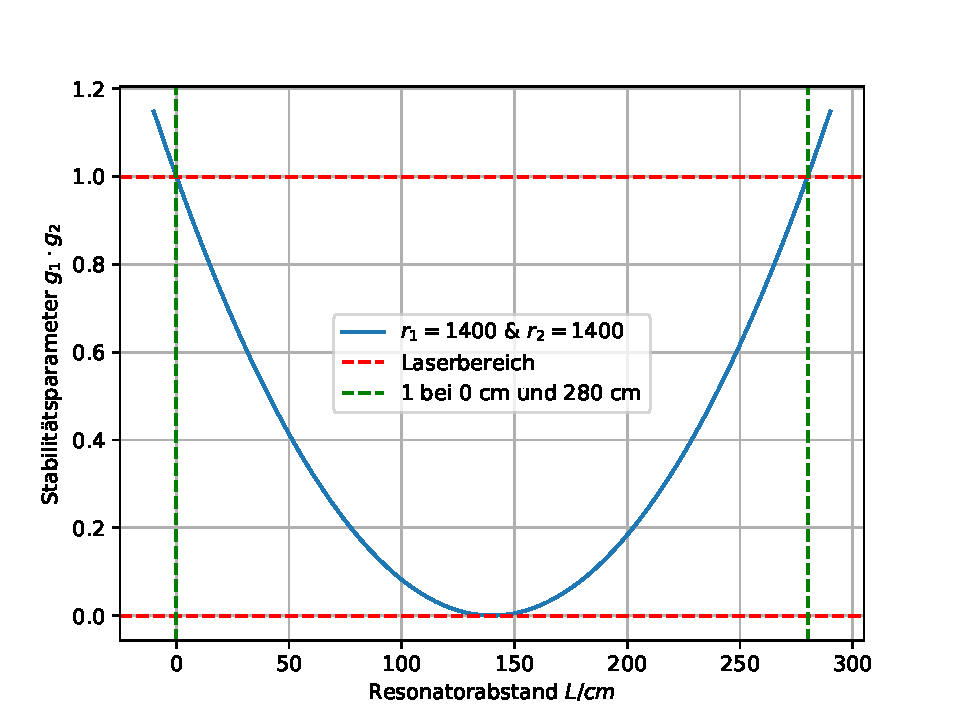
\includegraphics{plots/Vorbereitungsplot2.pdf}
  \caption{Theoretische Berechnung der Stabilitätsbedingung für die erste
Konfiguration. Aufgetragen sind $g_1 \cdot g_2$ gegen die Resonatorlänge $L$.}
  \label{fig:Konfig1}
\end{figure}

\begin{figure}[H]
  \centering
  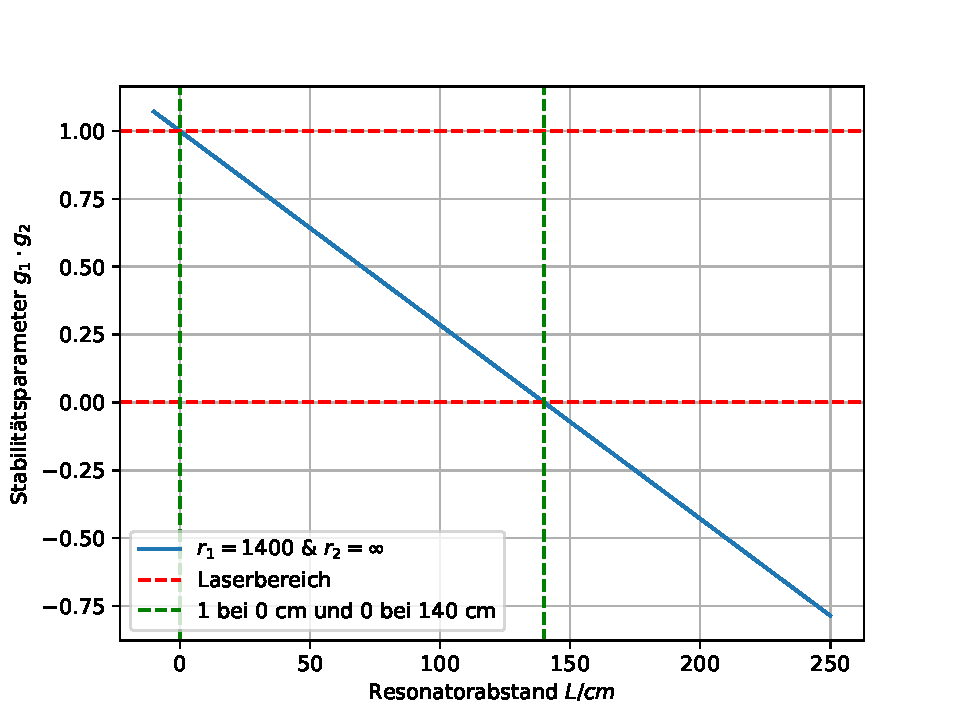
\includegraphics{plots/Vorbereitungsplot1.pdf}
  \caption{Theoretische Berechnung der Stabilitätsbedingung für die zweite Konfiguration. Aufgetragen sind
   $g_1 \cdot g_2$ gegen die Resonatorlänge $L$.}
  \label{fig:Konfig2}
\end{figure}

Im Experiment setzte die Lasertätigkeit bei den in Tabelle \ref{tab:Stabi} aufgeführten
Längen aus.
\begin{table}[H]
    \centering
    \caption{Im Experiment bestimmte maximale Rasonatorlängen für die Konfigurationen 1 und 2.}
    \label{tab:Konfig}
    \begin{tabular}{c|c}
        \toprule
        Konfiguration & $L_{\text{max}}$ in cm  \\
        \midrule
        1 & 191,7\\
        2& 116,7 \\
        \bottomrule
    \end{tabular}
\end{table}

\subsection{Vermessung zweier Moden}
Es werden die Grundmode $\symup{TEM}_{00}$ und die Mode $\symup{TEM}_{01}$ vermessen.
Aus der Formel \ref{eq:Elpq} lässt sich durch das einsetzen der Polynome für die jeweiligen
Parameter und bilden des Betragsquadrates die Intensität der Moden
\begin{align}
  I_{00}{x}&=I\cdot \exp{\left(-\frac{(x-x_{0})^{2}}{\sigma^{2}}\right)}\\
  I_{01}{x}&=I\cdot (x-x_{0})^{2} \exp{\left(-\frac{(x-x_{0})^{2}}{\sigma^{2}}\right)}
  \label{eq:Fit}
\end{align}
bestimmen.
Dabei ist $I$ die maximale Intensität, $x_0$ die Verschiebung der Funktion entlang der
x-Achse und $\sigma$ die Standartabweichung der Verteilung.\\
In den Abbildungen \ref{fig:M00} und \ref{fig:M01} sind die Daten aus Tabelle \ref{tab:DatenModen}
sowie die mittels Ausgleichsrechnung bestimmten Funktionen aus \ref{eq:Fit} dargestellt.
\begin{figure}[H]
  \centering
  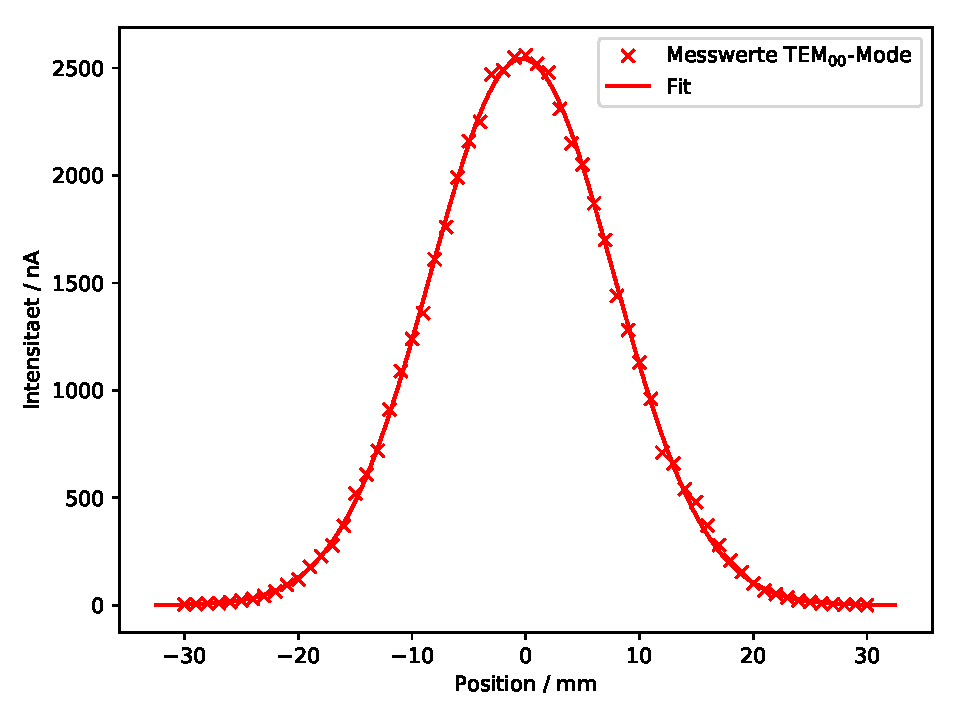
\includegraphics{plots/M00.pdf}
  \caption{Messwerte und Ausgleichskurve der $\text{TEM}_{00}$-Messung.}
  \label{fig:M00}
\end{figure}
Die Parameter für die 00-Mode ergeben sich zu:
\begin{align*}
  I &= (2543 \pm 8)\text{nm}\\
  x_0&=(-0.323 \pm 0.031) \text{mm}\\
  \sigma &= (-16.10 \pm 0.06) \text{mm}^{2}
\end{align*}

\begin{figure}[H]
  \centering
  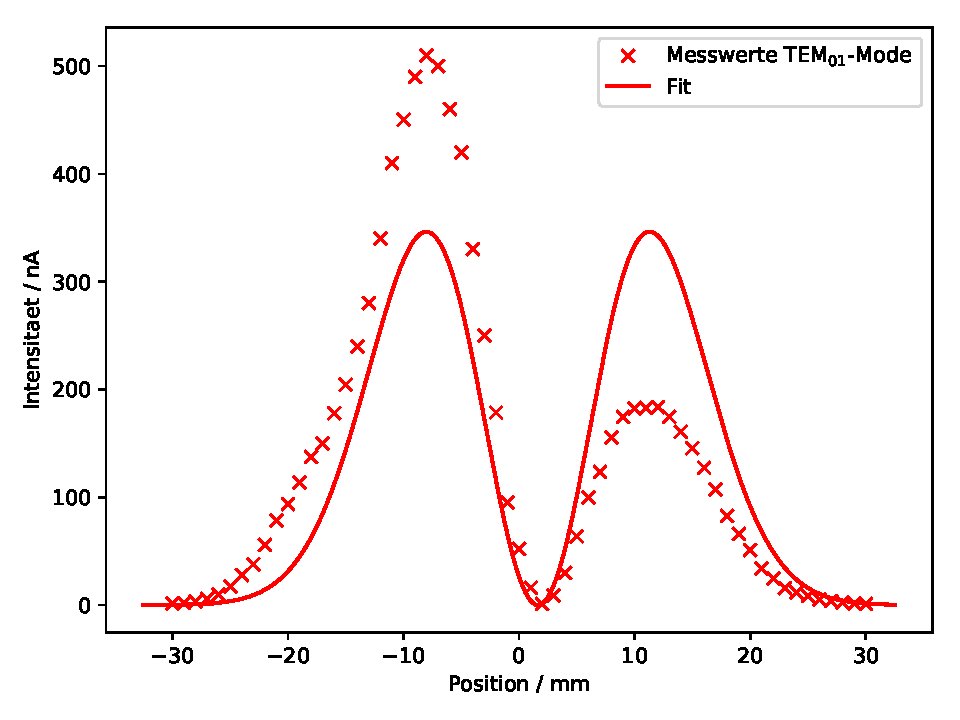
\includegraphics{plots/M01.pdf}
  \caption{Messwerte und Ausgleichskurve der $\text{TEM}_{01}$-Messung.}
  \label{fig:M01}
\end{figure}
Die Parameter für die 01-Mode ergeben sich zu:
\begin{align*}
  I &= (10.1\pm1.1)\text{nm}\\
  x_0&=(13.7\pm0.5) \text{mm}\\
  \sigma &= (1.6\pm0.4) \text{mm}^{2}
\end{align*}
\subsection{Polarisationsmessung}
Das Laserlicht ist nahezu perfekt linear polarisiert. Dies liegt an der Verwendung der
Brewsterfenster, welche nur den s-polatrisierten Lichtanteil reflektieren. Der
transmittierte Teil sowohl p- als auch s-polarisiertes Licht enthält. Durch die
mehrfachen Durchgänge durch die Brewsterfenster erleidet das s-polarisierte Licht
so große Verluste, dass der Intensitätsverlust gößer als der Gewinn ist, weshalb
das Laserlicht p-polarisiert ist.
Für die Intensitätsverteilunhg von linear polatrisiertem Licht, welches durch ein
Polarisationsfilter geht, gilt
\begin{equation}
  I(\phi)=I_0 \cos^2{\phi-\phi_0} .
\end{equation}
Dies wird Gesetz von Malus genannt,dabei wird eine Berücksichtigung einer Verschiebung $\phi_0$
mitbetrachtet.
Mit \ref{eq:Pola} wird eine Ausgleichsrechnung für die Polarisationsmessung durchgeführt.
In Abbildung \ref{fig:Pola} ist die resultierende Kurve sowie die Messwerte aufgetragen.
Die Parameter der Ausgleichsrechnung sind:
\begin{align*}
  I_0&=(11.4 \pm 1.1)\text{nA} \\
  phi_0&=(78 \pm 4)°
\end{align*}
\begin{figure}[H]
  \centering
  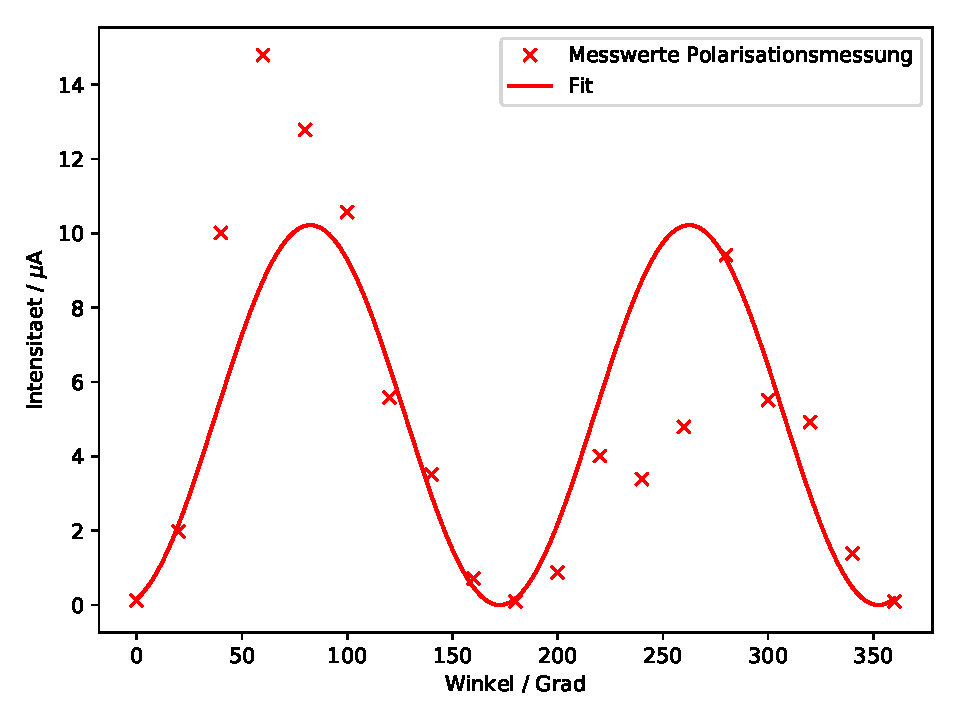
\includegraphics{plots/Polarisation.pdf}
  \caption{Messwerte und Ausgleichskurve der Polarisationsmessung.}
  \label{fig:Pola}
\end{figure}
\subsection{Wellenlängenuntersuchung}
Um die Wellenlänge des Lasers zu untersuchen, wird das Beugungsverhalten des Lichts an
einem Gitter untersucht. Das Gitter hat eine Gitterkonstante $g=0,01$mm$^{-1}$ und steht
$L=5,3$ cm vor der Photodiode.

In Abbildung \ref{fig:Welle} sind die Messwerte aufgetragen, wobei die Maxima farblich markiert sind. Mit
\begin{equation}
  \alpha = \tan{\frac{\Delta x}{L}}^{-1}
\end{equation}
werden die Abstäde zum Maximum bestimmt. Die Wellenlänge wird dann über
\begin{equation}
  \lambda=\frac{d\sin{\alpha}}{n}
  \label{eq:Welle}
\end{equation}
bestimmt.
Die Positionen der bestimmten Maxima sind in Tabelle \ref{tab:Max} aufgeführt.
\begin{table}[H]
    \centering
    \caption{Auflistung der Positionen der Maxima des Beugungsbild.}
    \label{tab:Max}
    \begin{tabular}{c|c|c|c|c|c|c|c}
        \toprule
        $x_1$& $x_2$ & $x_3$ & $x_4$ & $x_5$ & $x_6$ & $x_7$ & $x_8$\\
        \midrule
        10.0 mm & 6.5 mm & 3.0 mm & 0.0 mm & -4.0mm & -7.0mm & -11.0mm & -15.0mm \\
        \bottomrule
    \end{tabular}
\end{table}
\begin{figure}[H]
  \centering
  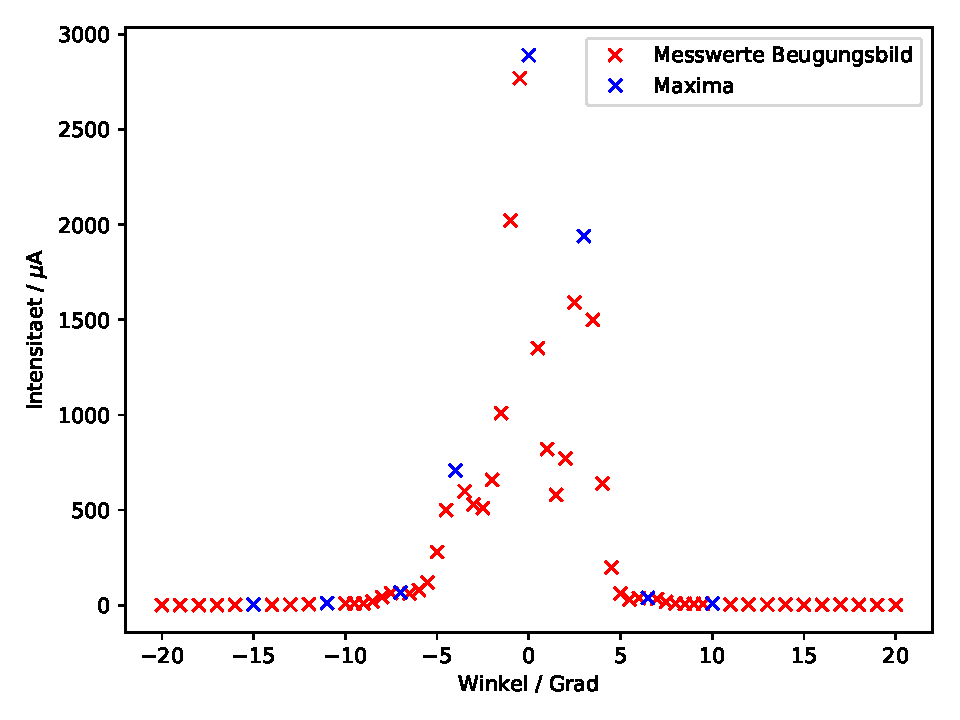
\includegraphics{plots/Wellenlaenge.pdf}
  \caption{Messwerte der Vermessung des Beugungsbildes, dabei sind die Maxima blau markiert.}
  \label{fig:Welle}
\end{figure}
Die mit \ref{eq:Welle} bestimmte Wellenlänge ist
\begin{equation*}
  \lambda= (646 \pm 27) \text{nm} .
\end{equation*}

\subsection{Multimodenuntersuchung}
Die gemessenen Peaks des Spektrum sind in Tabelle \ref{tab:Multi} zusammen mit den
gemittelten Peakabständen zufinden.
\begin{table}[h]
  \centering
  \caption{Peakpositionen für 3 Resonatorlängen, die Positionen sind in \si{MHz}
  angegeben.}
  \label{tab:Multi}
  \begin{tabular}{c | c c c c c c c c c c |c}
    \toprule
    $L$ / \si{\cm} & & & & & & & & & & & $\symup{\Delta}\nu$ / \si{MHz}\\
    \midrule
    \num{54.1} & 75 & 199& 274& 353& 473& 548& 623& 746 & -& -& $96\pm 9$\\
    \num{105.5} & 143& 281& 424& 566& 705& 848& 986& 1129 & -& - & $140.9\pm0.9$\\
    \num{195.5} & 79& 158& 236& 315& 394& 473& 551& 626& 705& 784&$78.3\pm0.4$ \\
    \bottomrule
  \end{tabular}
\end{table}
Bei Lichtgeschwindigkeit gilt eine Dopplerverschiebung von
\begin{equation}

\label{eq:Doppler}
\end{equation}
